\documentclass[tikz,border=10pt]{standalone}
\begin{document}
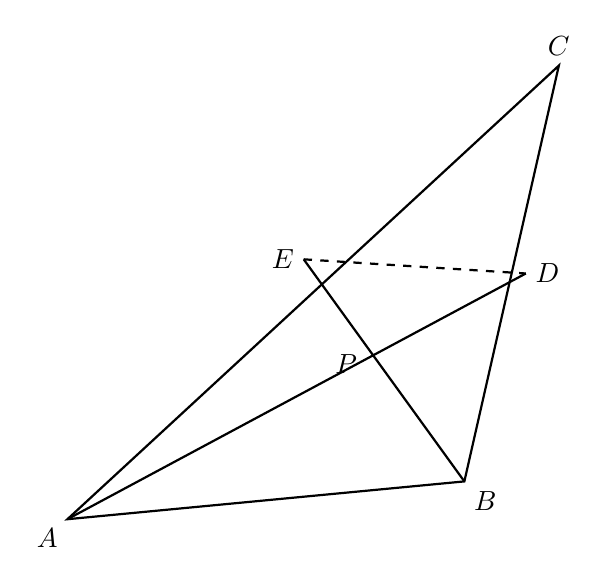
\begin{tikzpicture}[scale=1.2]
\coordinate (A) at (0,0);
\coordinate (B) at (4.2,0.4);
\coordinate (C) at (5.2,4.8);
\coordinate (D) at (4.85,2.6);
\coordinate (E) at (2.5,2.75);
\coordinate (P) at (2.95,1.85);

\draw[thick] (A) -- (B) -- (C) -- cycle;
\draw[thick] (A) -- (D);
\draw[thick] (B) -- (E);
\draw[dashed,thick] (E) -- (D);

\node[below left] at (A) {$A$};
\node[below right] at (B) {$B$};
\node[above] at (C) {$C$};
\node[right] at (D) {$D$};
\node[left] at (E) {$E$};
\node[below] at (P) {$P$};
\end{tikzpicture}
\end{document}
